\documentclass[letterpaper]{article}
\usepackage{natbib}
\usepackage[utf8]{inputenc}
\usepackage[margin=3.5cm]{geometry}
\usepackage{listings}
\usepackage{adjustbox}
\usepackage{xcolor}
\usepackage{verbatim}
\usepackage{graphicx}%images
\usepackage{fancyhdr}%for headers and footers
\usepackage{adjustbox}
\usepackage{verbatim}
\usepackage{listings}
\usepackage{fancyhdr}
\usepackage{multirow}
\usepackage{amsmath}
\usepackage{array}
\usepackage{mathpazo}
\usepackage{subcaption}
\usepackage{float}
\usepackage{csvsimple}
\usepackage{filecontents}
\usepackage{lscape}
\usepackage{afterpage}
\usepackage{hyperref}
\usepackage{inconsolata}
\usepackage{color}

\definecolor{pblue}{rgb}{0.13,0.13,1}
\definecolor{pgreen}{rgb}{0,0.5,0}
\definecolor{pred}{rgb}{0.9,0,0}
\definecolor{pgrey}{rgb}{0.46,0.45,0.48}

\lstset{language=Java,
  showspaces=false,
  showtabs=false,
  breaklines=true,
  showstringspaces=false,
  breakatwhitespace=true,
  commentstyle=\color{pgreen},
  keywordstyle=\color{pblue},
  stringstyle=\color{pred},
  basicstyle=\ttfamily,
  moredelim=[il][\textcolor{pgrey}]{$ $},
  moredelim=[is][\textcolor{pgrey}]{\%\%}{\%\%}
}



\hypersetup{
    colorlinks,
    citecolor=black,
    filecolor=black,
    linkcolor=black,
    urlcolor=black
}


% ------ HEADERS AND FOOTERS -----------
% \lhead{INFO-F403}
% \rhead{Project Report - Part 1}
%\pagestyle{fancy}
% \rfoot{\thepage}
%\cfoot{}
%\lfoot{Academic Year 2017-18}

\newcommand{\HRule}{\rule{\linewidth}{0.5mm}} %newcommand for cover page

\begin{document}
\begin{titlepage}
\begin{center}


\textsc{\LARGE universit\'e libre de bruxelles}\\[1.0cm]
\textsc{\Large D\'epartment d'Informatique}\\[1.5cm]

% Upper part of the page. The '~' is needed because \\
% only works if a paragraph has started.

\includegraphics[width=0.3\textwidth]{image/ulblogo.jpg}~\\[1cm]

\textsc{
\large INFO-F403 \\
\Large  Introduction to language theory and compiling
 \\[1cm]}
% Title
\HRule \\[0.7cm]

{ \huge \bfseries Project Report – Part 3  \\[0.7cm] }

\HRule \\[2cm]

% Author and supervisor
\noindent
\begin{center} \large

\emph{Author:}\\
\Large Hakim \textsc{Boulahya}\\
\end{center}
\begin{center} \large

% \emph{Professor:} \\
% Gilles \textsc{Geeraerts}\\

\end{center}

\vfill

% Bottom of the page
{\large \today}

\end{center}
\end{titlepage}

\tableofcontents
\newpage

\section{Introduction}

\paragraph{}

As part of the course of \textit{Introduction to Language theory and Compiling}
we were asked to
write a compiler of the IMP language. The goal of the third part of the
project was to implement the \textit{code generatar}.

\section{Parser Improvements}

\paragraph{}

To make the code generation easier to implement, the parser was modified
to produce an AST (abstract syntax tree).

To do so, some modification were make on the parser of part 2. The
derivation tree is constructed during the parsing \textit{i.e.} using
the stack implementation. The AST a post-process function, that modify
the derivation tree. The method \texttt{LL1Parser.buildAST()} simplifies
the derivation tree.

To simplify the derivation tree to an AST, \textit{simplifying} methods
has been implemented in \texttt{LL1Parser}. The resulitng
format of the AST are shown in the Figures below.
The trees
must be read from to bottom \textit{i.e.} the topmost
node is considered as the leftmost node.


\begin{figure}[H]
    \begin{subfigure}{.5\textwidth}
        \begin{lstlisting}
        begin
            print(x);
            x := 1
        end
        \end{lstlisting}
    \end{subfigure}
    \begin{subfigure}{.5\textwidth}
    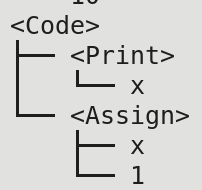
\includegraphics[scale=0.5]{image/code.png}
    \end{subfigure}
    \caption{Code AST: the format is a node $<$Code$>$ with children
    that are instructions}
\end{figure}

\begin{figure}[H]
    \begin{subfigure}{.5\textwidth}
        \begin{lstlisting}
        x := (1 + 2) * 5 / 1;
        \end{lstlisting}
    \end{subfigure}
    \begin{subfigure}{.5\textwidth}
    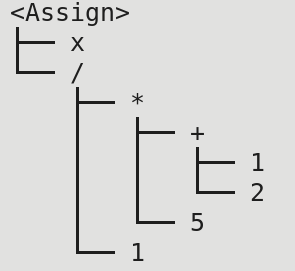
\includegraphics[scale=0.5]{image/assign.png}
\end{subfigure}
    \caption{Assign AST: The first child is the var name, and the second
    child an arithmetic expression.}
\end{figure}

\begin{figure}[H]
    \begin{subfigure}{.5\textwidth}
        \begin{lstlisting}
        x := -(2 - 1);
        \end{lstlisting}
    \end{subfigure}
    \begin{subfigure}{.5\textwidth}
    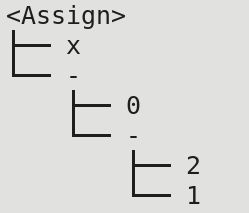
\includegraphics[scale=0.5]{image/neg-assign.png}
\end{subfigure}
    \caption{Negative arithmetic expressions: a minus in front of an
    expressions will be considered as a subtraction between 0 and expression.}
\end{figure}

\begin{figure}[H]
    \begin{subfigure}{.5\textwidth}
        \begin{lstlisting}
        print(x)
        read(c)
        \end{lstlisting}
    \end{subfigure}
    \begin{subfigure}{.5\textwidth}
    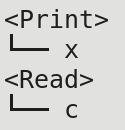
\includegraphics[scale=0.5]{image/print-read.png}
\end{subfigure}
    \caption{Print/Read AST: the variable name is the only child of those
    expression.}
\end{figure}

\begin{figure}[H]
    \begin{subfigure}{.5\textwidth}
        \begin{lstlisting}
        for i from 0 by 1 to 10 do
            x := x + 2
        done
    \end{lstlisting}
    \end{subfigure}
    \begin{subfigure}{.5\textwidth}
    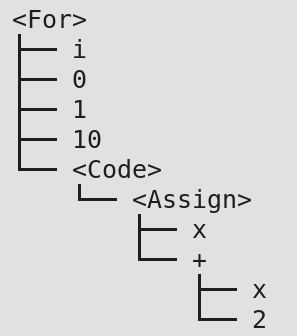
\includegraphics[scale=0.5]{image/for.png}
\end{subfigure}
    \caption{For AST: The first child is varname. The second child the
    initial value, third child the step (when not specified, it is 1),
    the fourth child is the maximum value. The last child is the code
    AST to execute if the condition are respected.}
\end{figure}

\begin{figure}[H]
    \begin{subfigure}{.5\textwidth}
        \begin{lstlisting}
        while i <= 10 do
            print(x);
            x := 1
        done
        \end{lstlisting}
    \end{subfigure}
    \begin{subfigure}{.5\textwidth}
    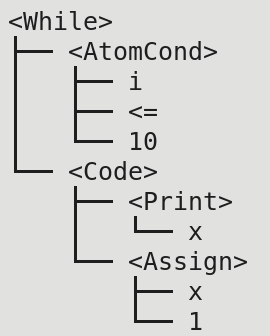
\includegraphics[scale=0.5]{image/while.png}
    \end{subfigure}

    \caption{While AST: The first child is the condition and the
    second child is the code AST to execute if the condition is true.}
\end{figure}

\begin{figure}[H]
    \begin{subfigure}{.5\textwidth}
        \begin{lstlisting}
        if x <> 1 and x < 10
           or z = 1 then

            print(x)
        else
            print(z)
        endif;
        \end{lstlisting}
    \end{subfigure}
    \begin{subfigure}{.5\textwidth}
    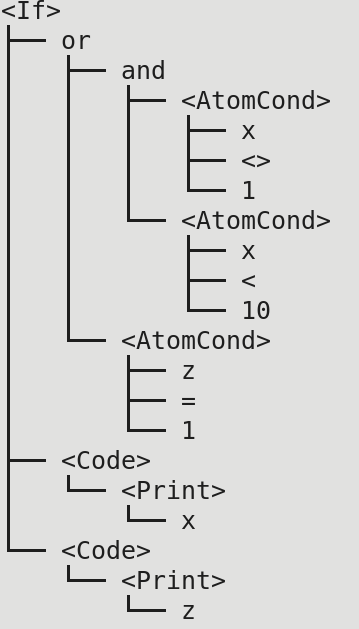
\includegraphics[scale=0.5]{image/if.png}
    \end{subfigure}
    \caption{If AST: The first child is the condition. The condition as
    follow the same simplification as the arithmetic expression, so that
    the priority of \texttt{or} and \texttt{and} are respected. The
    two last child are: the code AST to execute if the condition is true,
    and the code to execute if the code is false
     (\textit{i.e.} the else block)}.
\end{figure}

\section{Code generation}

\paragraph{}

The code generation consists in transforming the resulting AST into
LLVM IR code. The implementation of the code generation is in the
classe \texttt{CodeGenerator}. The initial AST is a code node \textit{i.e.}
an AST with children that represent each an instruction. Each type of
instruction are converted into specific instructions. Those following
decisions were made when generating the LLVM IR:

\begin{itemize}
    \item There is only one scope (since there is no function)
    \item An $<$If$>$ with
    two empty blocks will not generated any LLVM IR code
    \item The \texttt{not} condition
    instructions has been implemented in the AST directly. This means that
    the booleon operation is switched if the \texttt{not} keyword is used.
    Example: not a $<>$ b will create an instruction $a = b$.
    \item The memory allocation of a variable is called only once.
    It is allocated when the variable is first encountered in the AST.
    This means that the if, while, for blocks uses the same scope \textit{i.e.}
    assigning a variable inside a if will be accessible outside.

\end{itemize}

Figure below shows different IMP code and the corresponding generated
LLVM IR:

\begin{figure}[H]
    \begin{subfigure}{.5\textwidth}
        \begin{lstlisting}
        begin
            x := 1;
            print(x)
        end
        \end{lstlisting}
    \end{subfigure}
    \begin{subfigure}{.5\textwidth}
        \begin{lstlisting}
        ; T(<Assign>)
    	%1 = add i32 0, 1
    	%x = alloca i32
    	store i32 %1, i32* %x
        call void @println(i32* %x)
    	ret void
        \end{lstlisting}
    \end{subfigure}
    \caption{Example of basic allocation and print}
\end{figure}


\begin{figure}[H]
    \begin{subfigure}{.5\textwidth}
        \begin{lstlisting}
        while i <= 10 do
            print(x);
            x := 1
        done
        \end{lstlisting}
    \end{subfigure}
    \begin{subfigure}{.5\textwidth}
        \begin{lstlisting}
        ; T(<While>)loopCount=1
    	%1 = load i32, i32* %i
    	%2 = icmp sle i32 %1, 10
    	br i1 %2, label %beginLoop1, label %endLoop1
    	beginLoop1:
    	call void @println(i32* %x)
    	; T(<Assign>)
    	%3 = add i32 0, 1
    	%x = alloca i32
    	store i32 %3, i32* %x
    	%4 = load i32, i32* %i
    	%5 = icmp sle i32 %4, 10
    	br i1 %5, label %beginLoop1, label %endLoop1
    	endLoop1:
    	ret void
        \end{lstlisting}
    \end{subfigure}
     \caption{While loop example}
\end{figure}


\begin{figure}[H]
    \begin{subfigure}{.5\textwidth}
        \begin{lstlisting}
        for i from 0 by 1 to 10 do
            x := x + 2
        done
        \end{lstlisting}
    \end{subfigure}
    \begin{subfigure}{.5\textwidth}
        \begin{lstlisting}
        ; T(<For>)loopCount=1
    	%1 = add i32 0, 0
    	%i = alloca i32
    	store i32 %1, i32* %i
    	%2 = add i32 0, 10
    	%3 = load i32, i32* %i
    	%4 = icmp  slt i32 %3, %2
    	br i1 %4, label %beginLoop1, label %endLoop1
    	beginLoop1:
    	; T(<Assign>)
    	%5 = load i32, i32* %x
    	%6 = add i32 0, %5
    	%7 = add i32 0, 2
    	%8 = add i32 %6, %7
    	%x = alloca i32
    	store i32 %8, i32* %x
    	%9 = add i32 0, 1
    	%10 = load i32, i32* %i
    	%11 = add i32 %10, %9
    	store i32 %11, i32* %i
    	%12 = add i32 0, 10
    	%13 = load i32, i32* %i
    	%14 = icmp  slt i32 %13, %12
    	br i1 %14, label %beginLoop1, label %endLoop1
    	endLoop1:
    	ret void
        \end{lstlisting}
    \end{subfigure}
    \caption{For loop example. Not that the condition must be present
    before the beginLoop label, and in the block.}
\end{figure}


\begin{figure}[H]
    \begin{subfigure}{.5\textwidth}
        \begin{lstlisting}
        x := (1 + 2) * 5 / 1
        \end{lstlisting}
    \end{subfigure}
    \begin{subfigure}{.5\textwidth}
        \begin{lstlisting}
        %1 = add i32 0, 1
    	%2 = add i32 0, 2
    	%3 = add i32 %1, %2
    	%4 = add i32 0, 5
    	%5 = mul i32 %3, %4
    	%6 = add i32 0, 1
    	%7 = sdiv i32 %5, %6
    	%x = alloca i32
    	store i32 %7, i32* %x
    	ret void
        \end{lstlisting}
    \end{subfigure}
    \caption{Example of an arithmetic assignment}
\end{figure}


\begin{figure}[H]
    \begin{subfigure}{.5\textwidth}
        \begin{lstlisting}
        if x <> 1 and x < 10
           or z = 1 then
            print(x)
        else
            print(z)
        endif;
        \end{lstlisting}
    \end{subfigure}
    \begin{subfigure}{.5\textwidth}
        \begin{lstlisting}
        ; T(<If>)ifCount=1
    	%1 = load i32, i32* %x
    	%2 = icmp ne i32 %1, 1
    	%3 = load i32, i32* %x
    	%4 = icmp slt i32 %3, 10
    	%5 = add i1 %2, %4
    	%6 = icmp  eq i1 %5, 2
    	%7 = load i32, i32* %z
    	%8 = icmp eq i32 %7, 1
    	%9 = add i1 %6, %8
    	%10 = icmp  uge i1 %9, 1
    	br i1 %10, label %iftrue1, label %iffalse1
    	iftrue1:
    	call void @println(i32* %x)
    	br label %ifcontinue1
    	iffalse1:
    	call void @println(i32* %z)
    	br label %ifcontinue1
    	ifcontinue1:
    	ret void
        \end{lstlisting}
    \end{subfigure}
    \caption{If example. Note that the jump to the ifcontinue label must
    also be done in the else scope \textit{i.e.} in the iffalse label.}
\end{figure}

\end{document}
